\chapter{Sviluppo software}
\label{cap:sviluppo software}

% \intro{Breve introduzione al capitolo}\\

\section{Il progetto in partenza}
Il software nasceva come POC, era un monolite unico dove backend e frontend risiedevano nella stessa directory.\\
Il backend è scritto in python e si occupa di:
\begin{itemize}
    \item esporre un endpoint per il frontend 
    \item realizzare calcoli di machine learning per generare le visualizzazioni 
\end{itemize}

Il frontend invece era composto da tre due file html, uno per il form e uno per la visualizzazione dei grafici, due file javascript, uno per la validazione del form e uno per la realizzazione dei grafici, e un file css che dava lo stile a tutto. 

\section{Analisi e motivazioni}

Dopo una prima analisi del software ho proposto di operare una divisione più netta di front end e backend avvalendomi dell'ausilio di un framework per il frontend. Attraverso questa scelta si è seguito il principio di progettazione architetturale noto come \textit{Architettura a Strati} o \textit{Architettura a Livelli} (Layered Architecture).

Nell'architettura a strati, l'applicazione è suddivisa in diversi strati logici o livelli, ognuno dei quali ha una responsabilità specifica. Nel mio caso:
\begin{enumerate}
\item Backend (Strato logico):
    \begin{itemize}
        \item  Responsabilità: Gestisce la logica di presentazione, in particolare la generazione delle risposte API per il frontend.
        \item  Tecnologie utilizzate: Flask, Python, API REST.
    \end{itemize}
\item Frontend (Strato di Presentazione):
 \begin{itemize}
    \item Responsabilità: Interagisce con l'utente e invia richieste API al backend per ottenere e visualizzare i dati.
    \item Tecnologie utilizzate: React, JavaScript, HTML, CSS.
    \end{itemize}
\end{enumerate}
Questa separazione ha consentito di ottenere la divisione delle responsabilità, ovvero i livelli sono indipendenti l'uno dall'altro, facilitando la manutenzione e l'aggiornamento dei singoli componenti senza influenzare gli altri.\\

Dividere i due moduli e utilizzare un framework permette anche di semplificare gli sviluppo per il frontend, in particolare nel caso in futuro si volesse applicare moduli di registrazione e login, quindi avere cura della sicurezza, oppure ampliare il numero di grafici da mostrare all'utente. \\


\section{Sviluppi}
Gli sviluppi sono proseguiti in parallelo tra me e i colleghi che ho assistito. Io mi sono occupata principalmente del frontend, sono partita dall'interfaccia del wizard mentre ho assistito i colleghi nella realizzazione di endpoint e sistemazione del backend.\\
Dapprima sono stati realizzati endpoint separati che facessero la validazione e poi il submit del form, successivamente su mia sollecitazione le logiche sono state accorpate in un unico endpoint affinchè rispondesse con la visualizzazione oppure elencasse i campi non validi. Per quanto riguarda la validazione è stato eseguito un doppio controllo sia lato frontend sia lato backend, allo scopo di avere maggiore robustezza.\\

Il frontend è stato sviluppato in React, in particolare le librerie usate sono state:
\begin{itemize}
    \item Bootstrap per lo stile e alcuni componenti preconfezionati
    \item axios per le chiamate API
    \item toastify per mostrare toast multipli in fase di validazione del form del paziente
\end{itemize}

Ho avuto modo di operare piccole modifiche anche al backend, in particolare nella risposta tornata al frontend per calcolare le visualizzazioni. In origine infatti tra i campi modificabili vi era l'età, tuttavia a seguito di analisi si è concluso che non era una dimensione che potesse destare l'interesse del medico, quindi si è deciso di sostituirlo con il peso. In tal modo quindi il medico a frontend può verificare se il paziente, qualcosa aumentasse o diminuisse di peso, avrebbe una migliore risposta all'operazione oggetto della discussione.\\ 
Ho inoltre predisposto la POST degli endpoint che ricevono i form di valutazione dell'utente, in modo tale che il collega potesse successivamente sviluppare le feature per il salvataggio a csv del form compilato.\\ 

\section{Validazione}
La validazione merita una menzione a parte. Il software opera una doppia validazione: una lato frontend quando l'utente compila i campi, in modo tale da avere subito feedback se qualcosa non è corretto; questa viene fatta tramite chiamata a funzioni di validazioni implementate inizialmente dalla collega e successivamente evolute da me perchè funzionanti con React. Una lato backend, il quale controlla il form pervenuto e verifica se sia tutto conforme.\\
Se lato frontend non dovessero esserci segnalazioni di errori, ma al contrario il backend dovesse rispondere con un errore, questo viene notificato al frontend e l'utente può vedere a video una pagina di errore con la descrizione dell'errore. Nel caso in cui il backend dovesse rispondere errore 500 l'utente vedrà una pagina di errore con descrizione generica. 

\section{La struttura}
Le pagine principali sono le seguenti:\\ 
\begin{itemize}
\item Wizard: è presente il wizard iniziale dove l'utente compila i dati del paziente; si compone di 2 step dopo il primo è la scelta della zona da operare, il secondo è l'effettivo inserimento manuale dei dati
\item Evaluation: è la pagina di valutazione dell'applicativo, dove è presente un form che l'utente può compilare per darci il suo feedback. 
\item Tutorial: è una pagina accessibile dall' header che descrive l'applicativo e funge appunto da tutorial per l'utente. 
\end{itemize}
All'interno di queste pagine è possibile trovare diversi componenti necessari a suddividere ulteriormente la complessità delle pagine e delle logiche.\\ 
Abbiamo quindi il componente per l'header, gli step del wizard, il contenuto della dialog.\\

Nota importante è l'utilizzo del global context, ovvero un contesto globale che permette di condividere informazioni tra i diversi componenti senza dover sottostare per forza alla relazione parent-child. All'interno del global context possiamo trovare la gestione degli step, gran parte del form del wizard compilato dall'utente in quanto molte informazioni sono necessarie in più pagine e componenti, i dati fetchati in quanto servono alla pagina Results per calcolare le visualizzazioni. In particolare il global context si occupa di controllare anche se parte di questi dati sono già presenti nel local storage del browser, quindi di inizializzare le rispettive strutture dati. 


% Per lo studio dei casi di utilizzo del prodotto sono stati creati dei diagrammi.
% I diagrammi dei casi d'uso (in inglese \emph{Use Case Diagram}) sono diagrammi di tipo \gls{uml} dedicati alla descrizione delle funzioni o servizi offerti da un sistema, così come sono percepiti e utilizzati dagli attori che interagiscono col sistema stesso.
% Essendo il progetto finalizzato alla creazione di un tool per l'automazione di un processo, le interazioni da parte dell'utilizzatore devono essere ovviamente ridotte allo stretto necessario. Per questo motivo i diagrammi d'uso risultano semplici e in numero ridotto.

% \begin{figure}[!h] 
%     \centering 
%     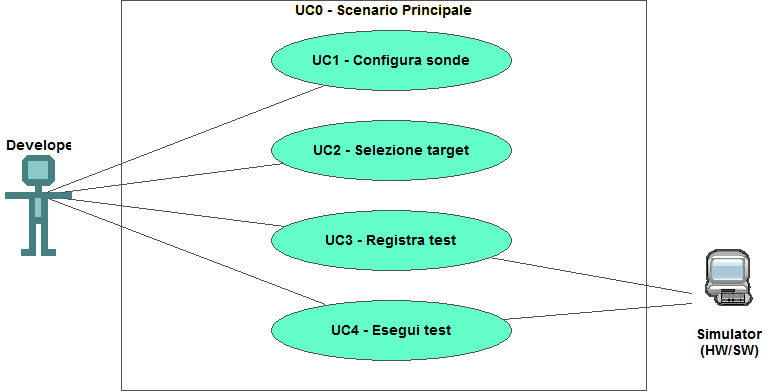
\includegraphics[width=0.9\columnwidth]{usecase/scenario-principale} 
%     \caption{Use Case - UC0: Scenario principale}
% \end{figure}

% \begin{usecase}{0}{Scenario principale}
% \usecaseactors{Sviluppatore applicativi}
% \usecasepre{Lo sviluppatore è entrato nel plug-in di simulazione all'interno dell'IDE}
% \usecasedesc{La finestra di simulazione mette a disposizione i comandi per configurare, registrare o eseguire un test}
% \usecasepost{Il sistema è pronto per permettere una nuova interazione}
% \label{uc:scenario-principale}
% \end{usecase}

% \section{Tracciamento dei requisiti}

% Da un'attenta analisi dei requisiti e degli use case effettuata sul progetto è stata stilata la tabella che traccia i requisiti in rapporto agli use case.\\
% Sono stati individuati diversi tipi di requisiti e si è quindi fatto utilizzo di un codice identificativo per distinguerli.\\
% Il codice dei requisiti è così strutturato R(F/Q/V)(N/D/O) dove:
% \begin{enumerate}
% 	\item[R =] requisito
%     \item[F =] funzionale
%     \item[Q =] qualitativo
%     \item[V =] di vincolo
%     \item[N =] obbligatorio (necessario)
%     \item[D =] desiderabile
%     \item[Z =] opzionale
% \end{enumerate}
% Nelle tabelle \ref{tab:requisiti-funzionali}, \ref{tab:requisiti-qualitativi} e \ref{tab:requisiti-vincolo} sono riassunti i requisiti e il loro tracciamento con gli use case delineati in fase di analisi.

% \newpage

% \begin{table}%
% \caption{Tabella del tracciamento dei requisti funzionali}
% \label{tab:requisiti-funzionali}
% \begin{tabularx}{\textwidth}{lXl}
% \hline\hline
% \textbf{Requisito} & \textbf{Descrizione} & \textbf{Use Case}\\
% \hline
% RFN-1     & L'interfaccia permette di configurare il tipo di sonde del test & UC1 \\
% \hline
% \end{tabularx}
% \end{table}%

% \begin{table}%
% \caption{Tabella del tracciamento dei requisiti qualitativi}
% \label{tab:requisiti-qualitativi}
% \begin{tabularx}{\textwidth}{lXl}
% \hline\hline
% \textbf{Requisito} & \textbf{Descrizione} & \textbf{Use Case}\\
% \hline
% RQD-1    & Le prestazioni del simulatore hardware deve garantire la giusta esecuzione dei test e non la generazione di falsi negativi & - \\
% \hline
% \end{tabularx}
% \end{table}%

% \begin{table}%
% \caption{Tabella del tracciamento dei requisiti di vincolo}
% \label{tab:requisiti-vincolo}
% \begin{tabularx}{\textwidth}{lXl}
% \hline\hline
% \textbf{Requisito} & \textbf{Descrizione} & \textbf{Use Case}\\
% \hline
% RVO-1    & La libreria per l'esecuzione dei test automatici deve essere riutilizzabile & - \\
% \hline
% \end{tabularx}
% \end{table}%
